\chapter{Úvod do problematiky}

Při řešení problémů hledáme způsob jak interpretovat data v takovém formátu, se kterým již umíme pracovat. Jedním ze základních prvků je matice. Ve spoustě případů takové matice obsahují nemalý počet nulových prvků.

Použití řídkých matic najdeme 2D/3D grafice, simulaci fyzikálních jevů ať už řešení úloh proudění tekutin, elektrické či meteorologické, statistice, pagerank a další.
TODO přeložit: computational fluid dynamics, finite-element methods, statistics, time/frequency 
domain circuit simulation, dynamic and static modeling of chemical processes, 
cryptography, magneto-hydrodynamics, electrical power systems, differential
equations, quantum mechanics, structural mechanics (buildings, ships, aircraft,
human body parts...), heat transfer, MRI reconstructions, vibroacoustics, linear 
and non-linear optimization, financial portfolio optimization, semiconductor 
process simulation, economic modeling, oil reservoir modeling, astrophysics, 
crack propagation,  Google page rank, 3D computer vision, cell phone tower 
placement, tomography, multibody simulation, model reduction, nano-technology, 
acoustic radiation, density functional theory, quadratic assignment, elastic 
properties of crystals, natural language processing, DNA electrophoresis, ... 

% see: https://www.youtube.com/watch?v=jECBfI52hk8

Pro výstavu v roce 2011 s názvem Art in Enginnering v Harnově Muzeu představila floridská univerzita kolekci s názvem The Beauty of Mathematics: As Illustrated by the University of Florida Sparse Matrix Collection. Pro estetické zobrazení řídkých matic byla provedena simulace. Každému uzlu byl přiřazen elektrický náboj a každá hrana představovala pružinu. V simulaci byla celá tato kontrukce položena na tvrdou podložku. Simulace byla zastavena, když se konstrukce přestala hýbat. Pro ilustraci přikládáme výsledek simlulace na modelu helikoptéry.

\begin{figure}[H]
	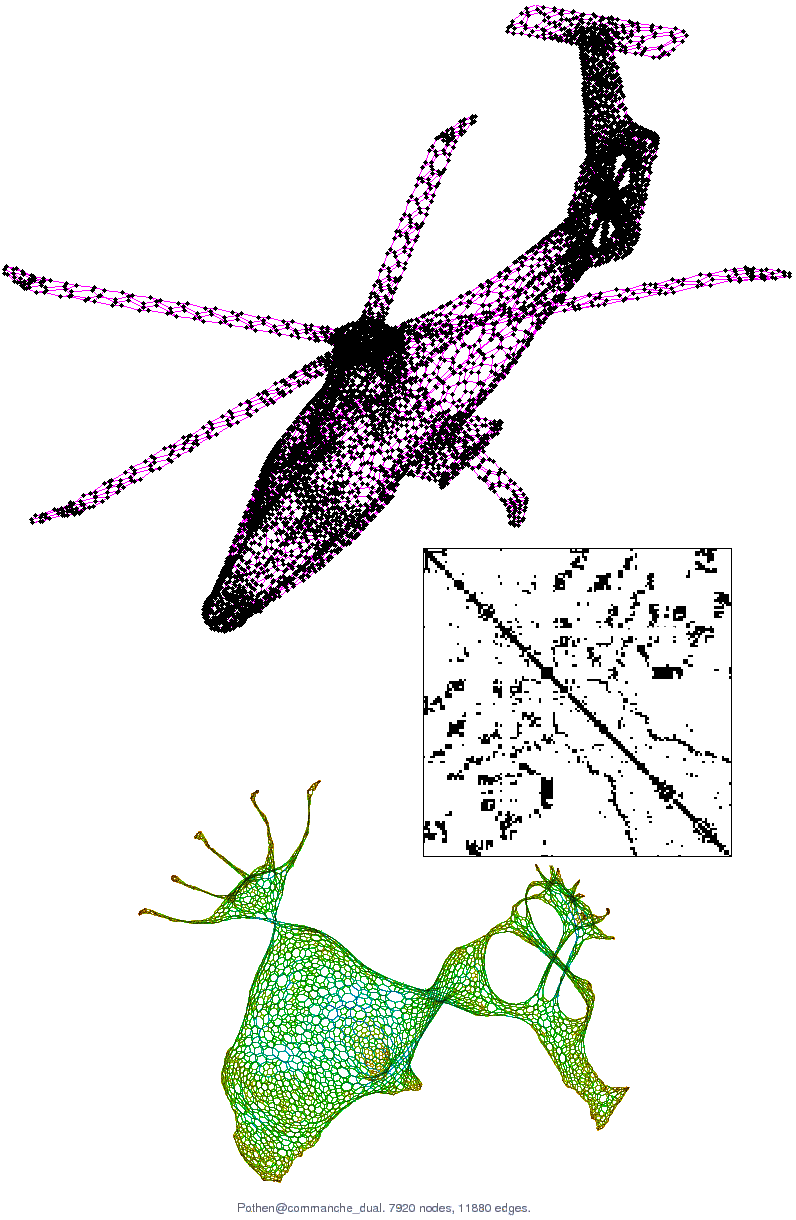
\includegraphics[width=1.0\textwidth]{./images/commanche/commanche}
	\caption{3D neorientovaný graf ve tvaru helikoptéry, jeho reprezentace v řídké matici a výsledek simulace}
	\label{fig:commanche}
\end{figure}

TODO:
To cite this collection, use the following: The University of Florida Sparse Matrix Collection T. A. Davis and Y. Hu, ACM Transactions on Mathematical Software, Vol 38, Issue 1, 2011, pp 1:1 - 1:25. \url{http://www.cise.ufl.edu/research/sparse/matrices}

\section{Použití násobení matic}

Metodou konečných prvků můžeme simulovat různé proudění, deformace a další fyzikální zákony
\url{Phttp://ocw.mit.edu/courses/materials-science-and-engineering/3-11-mechanics-of-materials-fall-1999/modules/fea.pdf}

Electric Impedance Tomography
\url{http://engineering.dartmouth.edu/~d22888z/documents/EIT_Bath_2011_v2.pdf}


Násobení matice maticí má menší praktické využití než násobení matice vektorem. V praxi ale můžeme složit více vektorů v jednu matici a tím si zrychlit výpočet. To se obzvlášťě hodí pro real-time aplikace.

%psal to tady: http://www.researchgate.net/post/Could_anybody_tell_me_some_models_or_applications_in_which_Sparse_Matrix_Matrix_Products_are_required3

% \url{http://math.stackexchange.com/questions/116717/can-a-basis-for-a-vector-space-be-made-up-of-matrices-instead-of-vectors}



\url{http://www.cise.ufl.edu/research/sparse/}

% inverze matic: Matrix multiplication and matrix inversion ItA

TODO: kde se pouziva nasobeni matic

\section{Matice}

Matice \textbf{A} typu ($m$, $n$) je $m n$ uspořádaných prkvů z množiny $\mathbf{R}$. O prvku $a_{r,s} \in \mathbf{R}, r \in \{1,2,\hdots,m\},s \in \{1,2,\hdots,n\}$ říkáme, že je na r-tém řádku a~s-tém sloupci matice \textbf{A}. Matici \textbf{A} zapisujeme do řádků a~sloupců takto:
\begin{align}
\mathbf{A}=\begin{pmatrix}
a_{1,1} & a_{1,2} & \cdots & a_{1,n} \\
a_{2,1} & a_{2,2} & \cdots & a_{2,n} \\
\vdots  & \vdots  & \ddots & \vdots  \\
a_{m,1} & a_{m,2} & \cdots & a_{m,n}
\end{pmatrix}
\end{align}

Matici \textbf{M} typu ($m$, $n$), kde všechny její prvky jsou rovny nule, nazýváme \textit{nulovou maticí.}

O~matici typu ($m$, $n$) budeme říkat, že je $m$~široká a~$n$~vysoká. Pokud o~matici řekneme že má velikost $n$, myslíme tím, že je typu ($n$, $n$).

\section{Vektor}

Matici \textbf{V} typu (1, n) nazveme vektorem.

\section{Násobení matice maticí}

Buď \textbf{A} matice typu ($m$,$n$) s prvky $a_{i,j}$ a \textbf{B} matice typu ($n$,$p$) s prvky $b_{j,k}$. Definujeme součin matic $\mathbf{A} \cdot \mathbf{B}$ jako matici \textbf{C} typu ($m$,$p$) s prvky $c_{i,k}$ které vypočteme jako:

\begin{align}
c_{row,col}=\sum_{k=1}^{N} a_{row,k} b_{k,col}
\end{align}

Výsledek součinu matic se nezmění, pokud matice doplníme o~libovolný počet nulových řádků a~nebo sloupců. Této vlastnosti můžeme využít pro získání potřebných rozměrů:

\begin{enumerate}
  \item Při násobení matice A typu ($m$,$n$) s maticí B typu ($o$,$p$), kde $ n \neq o $.
  \item Pokud potřebujeme matice stejné velikosti.
  \item Pokud potřebujeme matice určité velikosti, například $ 2^{ \mathbf{N}} $.
\end{enumerate}

Násobení matice vektorem je pouze případem násobení matice typu ($m$,$n$) s maticí typu ($n$,$1$).

\section{Složitosti}

TODO: popsat notace, mistrovskou metodu z: IntroductionToAlgoritms 3.1 asymptotic notations 43-97 (1217, 1222).

\section{Řídké matice}

Matice, které obsahují velké množství nulových prvků, nazýváme řídké. Nebudeme přesně uvádět, kolik procent z celkového počtu prvků musí být nulových, abychom matici nazývali řídkou. Stejně jako řídkou matici můžeme uložit do formátu pro husté matice, můžeme hustou matici uložit do formátu pro řídké matice.

Řídkost matice budeme vyjadřovat pomocí $nnz$ (Number of NonZero elements), tedy počtem nenulových prvků z celkových $mn$, pro matici A typu ($m$, $n$).

TODO: typy ridkych matic (pasova, atd, pattern, real)

\section{Numerická stabilita}

TODO: numerická stabilita obecne (viz strassen)

\section{Optimalizace kódu}

Dnešní překladače umí velice dobře optimalizovat vygenerovaný kód. Pokusy o nějaké mikrooptimalizace program spíše zpomalí.

Je vhodné používat funkce standartních knihoven, protože bývají optimalizované přímo v assembleru.

TODO: priklady, zdroje

\subsection{Rozděl a panuj}
divide, conquer, combine

\subsection{Rozbalování cyklů}

\subsection{AoS -> SoA}

\subsection{Loop tiling}

TODO: \url{https://edux.fit.cvut.cz/courses/BI-EIA/_media/lectures/kompilator.pdf}

%-----------------------------------------------------------------------------
%-----------------------------------------------------------------------------
%-----------------------------------------------------------------------------